% Name: Convolutional network
% Description: An image passing through convolution and pooling layers to a dense classifier, drawn as blocks.
% Tags: CNN, convolution, pooling, deep learning

\usetikzlibrary{arrows.meta}

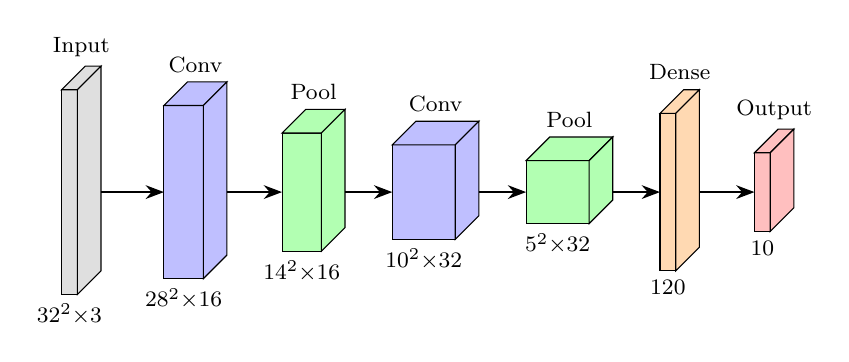
\begin{tikzpicture}[every node/.style={font=\footnotesize, align=center}]
  \foreach \x/\h/\w/\c/\name/\size in {
      0/2.6/0.2/gray!25/Input/$32^2{\times}3$,
      1.3/2.2/0.5/blue!25/Conv/$28^2{\times}16$,
      2.8/1.5/0.5/green!30/Pool/$14^2{\times}16$,
      4.2/1.2/0.8/blue!25/Conv/$10^2{\times}32$,
      5.9/0.8/0.8/green!30/Pool/$5^2{\times}32$,
      7.6/2/0.2/orange!30/Dense/$120$,
      8.8/1/0.2/red!25/Output/$10$%
  } {
    \draw[fill=\c] (\x,-\h/2) rectangle ++(\w,\h);
    \draw[fill=\c] (\x,\h/2) -- ++(0.3,0.3) -- ++(\w,0) -- ++(-0.3,-0.3) -- cycle;
    \draw[fill=\c] (\x+\w,-\h/2) -- ++(0.3,0.3) -- ++(0,\h) -- ++(-0.3,-0.3) -- cycle;
    \node[above] at (\x+\w/2+0.15,\h/2+0.3) {\name};
    \node[below] at (\x+\w/2,-\h/2) {\size};
  }
  \foreach \a/\b in {0.5/1.3, 2.1/2.8, 3.6/4.2, 5.3/5.9, 7/7.6, 8.1/8.8}
    \draw[-{Stealth}, thick] (\a,0) -- (\b,0);
\end{tikzpicture}
